\documentclass[11pt,xcolor={dvipsnames},usepdftitle=false]{beamer}
\usepackage{presentation}
\usepackage{makecell}
\usepackage{tabularx}
\usepackage{booktabs}
\usepackage{xcolor}

\hypersetup{pdfpagemode=UseNone,hidelinks,pdfdisplaydoctitle=true,%
%
% Enter presentation title to populate PDF metadata:
pdftitle={IoT Discovery Protocols: a MQTT-Discovery and UPnP Comparison}}

\definecolor{darkgreen}{RGB}{0, 103, 79}
\definecolor{mqttpurple}{RGB}{115, 38, 113}
\definecolor{upnpgreen}{RGB}{53, 219, 86}
\newcommand{\emphasise}[1]{{\textcolor{darkgreen}{\textbf{#1}}}}


\begin{document}

% Enter title:
\title{IoT Discovery Protocols:\\a MQTT-Discovery and UPnP Comparison}

\information%
%
% Enter URL to research paper (can be commented out):
[https://github.com/DaniDF/MQTT-Discovery-vs-UPnP/blob/main/docs/MQTTDiscovery\_vs\_UPnP.pdf]
%
% Enter authors:
{Daniele Foschi}

\frame{\titlepage}

% Enter content of presentation:
\begin{frame}{Background}
    % Due parole su IoT
    % Elenco protocolli più usati
    \emphasise{IoT}: \textit{A global infrastructure for the information society, enabling advanced services by interconnecting (physical and virtual) things based on existing and evolving interoperable information and communication technologies.} [I.T.U.]

    \vspace{3em}
    
    Large number of (different) devices require \emphasise{DISCOVERY} solutions.

    \vspace{3em}

    \begin{tabularx}{\textwidth}{@{}X X X@{}}
        \makecell[c]{\emphasise{WHERE}} & \makecell[c]{\emphasise{HOW}} & \makecell[c]{\emphasise{WHAT}} 
        \vspace{0.5em} \\
        \makecell[c]{\textit{are the devices?}} & \makecell[c]{\textit{to interact with them?}} & \makecell[c]{\textit{can they offer?}}
    \end{tabularx}
\end{frame}

\begin{frame}{MQTT-D vs UPnP}
    % Descrizione MQTT-D e UPnP a confronto
    %   Eplicitare che MQTT-D è basato su MQTT e cosa aggiunge
    %   dualismo client-server e pub-sub (gena)
    %   qos mx
    \centering
    \begin{tabular}{c|c|c}
        \centering
        & \emphasise{UPnP} & \emphasise{MQTT-D} \\ 
        \hline
        \emphasise{Architecture} & \makecell{Decentralized \\ (P2P)} & \makecell{Centralized \\ (Client-Broker)} \\
        \hline
        \makecell{\emphasise{Transport Protocol}} & \makecell{UDP Multicast \\ (HTTP over UDP)} & TCP/IP \\
        \hline
        \makecell{\emphasise{Network Scope}} & \makecell{Local \\ (LAN,  \\ Time-to-Live = 2)} & \makecell{Global \\ (not limited)} \\
        \hline
        \makecell{\emphasise{Data Format}} & XML & JSON \\
    \end{tabular}
    
\end{frame}

\begin{frame}{Proposition}
    % Descrivere cosa si vuole dimostrare: misurare le performance dei protocolli
    % Definire le metriche usate: latency and robustness
    Stress \emphasise{UPnP} and \emphasise{MQTT-D} \emphasise{discovery} and \emphasise{communication performances} in a highly \emphasise{dense network} environment.

    \vspace{2em}

    \begin{center}
        \emphasise{METRICS}
    \end{center}
    
    \vspace{1em}
    
    \begin{tabularx}{\textwidth}{@{}X X@{}}
        \makecell[c]{\emphasise{Latency}} & \makecell[c]{\emphasise{Robustness}} \\
        \makecell[c]{Time needed for the execution \\ of the first interaction between \\ control-point and device} & \makecell[c]{The ratio between discovered \\ devices and total deployed units}
    \end{tabularx}
\end{frame}

\begin{frame}{Experiment Setup}
    % Descrivere in che modo è stato effettuato l'esperimento
    % Foto setup
    \textcolor{blue}{TODO: foto setup}
    
    \emphasise{Two nodes}: one playing the role of \emphasise{\textit{device}} the other the role of \emphasise{\textit{control-point}} (a third plays the role of \emphasise{broker} for MQTT-D).

    \vspace{3em}

    \emphasise{TESTS}: scaled deployment of \textit{devices} and \textit{control-points} \emphasise{from 1 to 10} then from \emphasise{10 to 100 with decal increment}. Each configuration evaluated \emphasise{30 times}.
\end{frame}

\begin{frame}{Results - Comparison}
    % Mostrare una comparazione per latenza e una per robustness
    \begin{figure}[!ht]
        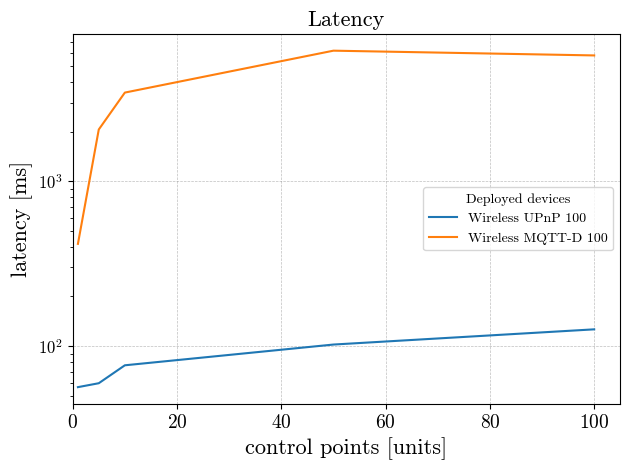
\includegraphics[width=0.47\linewidth]{images/mqtt-upnp_latency_light.png}
        \hfill
        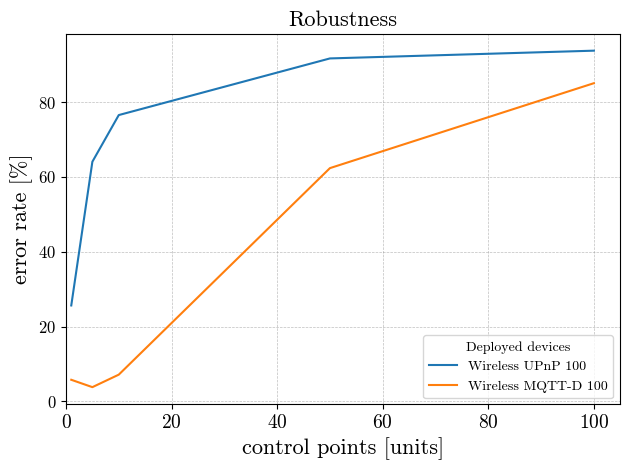
\includegraphics[width=0.47\linewidth]{images/mqtt-upnp_robustness_light.png}
    \end{figure}

    \emphasise{UPnP outperforms} MQTT-D in terms of \emphasise{latency} BUT it is \emphasise{less robust}.
\end{frame}

\begin{frame}{Results - Communication}
    % Mostrare una comparazione per wired wired
    \begin{figure}[!ht]
        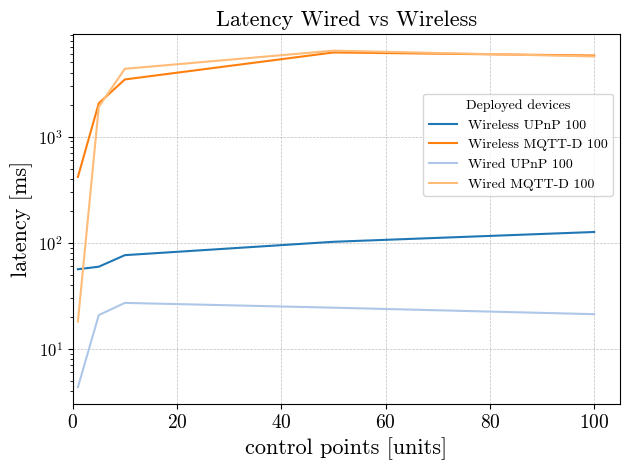
\includegraphics[width=0.47\linewidth]{images/wired-less_mqtt-upnp_latency_light.png}
        \hfill
        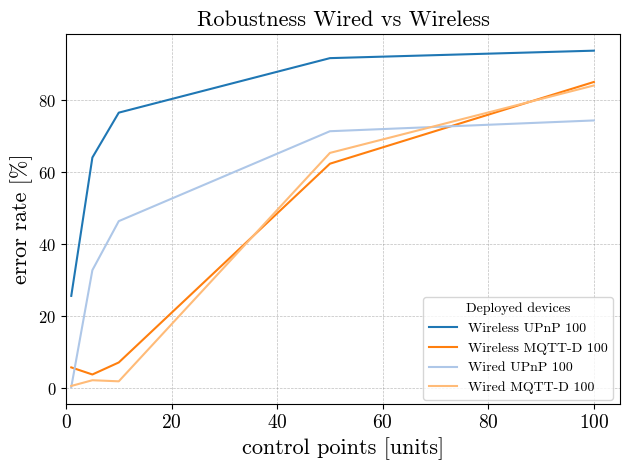
\includegraphics[width=0.47\linewidth]{images/wired-less_mqtt-upnp_robustness_light.png}
    \end{figure}

    Only \emphasise{UPnP benefits} from having a \emphasise{wired} connection, the performance difference in \emphasise{MQTT-D} is \emphasise{negligible}.
\end{frame}

\begin{frame}{Demonstration}
    % Mostrare foto di quello che si vuole far vedere dal vivo
    % Spiegare cosa si vedra: luce si accende per mqtt si spegne per UPnP
    % Mostrare i valori ottenuti e spiegarne velocemente il significato
    What we are going to see:
    \begin{enumerate}
        \item \emphasise{Initial state}: Led off
        \item \textcolor{mqttpurple}{MQTT-D}:

        \begin{enumerate}
            \item Connection to the MQTT Broker
            \item Subscribe to discovery topics
            \item Discovery of the available devices and their APIs
            \item RPC call: turn led on and measure the execution time
        \end{enumerate}

        \item \textcolor{upnpgreen}{UPnP}:

        \begin{enumerate}
            \item SSDP: discovery
            \item GENA: subscribe to every device
            \item SOAP: RPC call turn led off and measure the execution time
            \item GENA: receive state update and measure the elapsed time
        \end{enumerate}
        
    \end{enumerate}
\end{frame}

\begin{frame}{Future Work}
    % Ulteriori misurazioni spaziali e temporali come nel paper che hai trovato

    Some of the still open questions:
    
    \begin{itemize}
        \item \emphasise{Payload}: how does payload affects latency and robustness?
        \item \emphasise{Update}: how different version of IEEE 802.11 protocols affects the measurements?
        \item \emphasise{DTN}: how do these protocols work in disruptive networks?
    \end{itemize}
\end{frame}

\begin{frame}{Summary \& Thank You}

    \emphasise{Key Takeaways}
    \begin{enumerate}
        \item UPnP better latency
        \item MQTT-D better robustness
        \item UPnP is more affected by the connection technology than MQTT-D
    \end{enumerate}

    \vspace{2\baselineskip}

    \begin{center}
        \textit{\emphasise{Thank you, Questions welcome}}
    \end{center}
\end{frame}

\lastslide

\end{document}